\section{Stage 1B Full Dimension Sweep}
\label{app:stage1b}

Stage~1B tests whether the endpoint ranking signal preserved under random
projections in Stage~1A (Appendix~\ref{app:stage1a}) transfers to CEM
planning behavior.  We evaluate four protocol cells: PushT with full
projected CEM, PushT with re-rank-only selection, Cube with full projected
CEM, and Cube with re-rank-only selection.  Table~2 and Figure~3 in the
main text show representative dimensions; this appendix reports the full
dimension sweep and the subset structure behind those aggregate trends.

\subsection{PushT Full Projected CEM}
\label{app:stage1b_pusht_full}

\begin{table}[h]
\centering
\caption{PushT full projected CEM across projection dimensions.  The sweep
uses 63 Track~A pairs and three projection seeds per dimension.  Dashes mark
dimensions whose endpoint values are inherited from the Stage~1A C2 endpoint
sweep rather than directly emitted in the CEM gap table.}
\label{tab:g-pusht-full}
\small
\begin{tabular}{ccccc}
\toprule
$m$ & $\Rendpoint$ & $\Rpool$ & $\DeltaCEM$ & $M_{\text{rank1}}$ (\%) \\
\midrule
1 & 0.196 & 0.026 & 0.169 & 11.1 \\
2 & 0.235 & $-$0.027 & 0.262 & 13.8 \\
4 & 0.323 & 0.036 & 0.287 & 15.3 \\
8 & 0.379 & 0.080 & 0.299 & 20.6 \\
16 & 0.407 & 0.092 & 0.315 & 23.8 \\
32 & 0.444 & 0.111 & 0.333 & 28.0 \\
64 & 0.473 & 0.040 & 0.432 & 29.6 \\
128 & 0.477 & 0.051 & 0.426 & 30.7 \\
192 & 0.495 & 0.067 & 0.428 & 34.4 \\
\bottomrule
\end{tabular}
\end{table}

PushT full projected CEM success rises monotonically from 11.1\% at $m=1$
to 34.4\% at $m=192$, with a visible elbow between $m=8$ and $m=32$.
However, $\Rpool$ stays below 0.12 across all dimensions even as
$\Rendpoint$ rises to 0.495.  The widening $\DeltaCEM$ therefore confirms
the endpoint--planning decoupling from Section~4.

\subsection{PushT Re-rank-only}
\label{app:stage1b_pusht_rerank}

\begin{table}[h]
\centering
\caption{PushT re-rank-only projected selection.  Default CEM final pools
are fixed, simulator-scored, and then re-ranked by projected endpoint costs
over 100 pairs and three projection seeds.}
\label{tab:g-pusht-rerank}
\small
\begin{tabular}{cccccc}
\toprule
$m$ & $\Rendpoint$ & $\Rpool$ & $\DeltaCEM$ & $M_{\text{rank1}}$ (\%) & Pool success (\%) \\
\midrule
1 & 0.196 & 0.050 & 0.146 & 31.3 & 33.1 \\
8 & 0.379 & 0.073 & 0.306 & 33.0 & 33.1 \\
32 & 0.444 & 0.107 & 0.337 & 36.7 & 33.1 \\
64 & 0.473 & 0.079 & 0.394 & 35.3 & 33.1 \\
192 & 0.495 & 0.095 & 0.400 & 34.0 & 33.1 \\
\bottomrule
\end{tabular}
\end{table}

The re-rank-only $M_{\text{rank1}}$ varies by only 5.4 percentage points
across all dimensions, from 31.3\% to 36.7\%, confirming the flatness
reported in Section~4.  Pool success is constant at 33.1\% because the
default CEM pool is fixed.  The flat success curve despite rising
$\Rendpoint$ shows that final-pool re-ranking with projected costs adds
little over default selection.

\subsection{Cube Full Projected CEM}
\label{app:stage1b_cube_full}

\begin{table}[h]
\centering
\caption{Cube full projected CEM across representative dimensions.  The
final sweep uses 50 pairs and three projection seeds; all reported success
and pool-success values are percentages.}
\label{tab:g-cube-full}
\small
\begin{tabular}{cccccc}
\toprule
$m$ & $\Rendpoint$ & $\Rpool$ & $\DeltaCEM$ & $M_{\text{rank1}}$ (\%) & Pool success (\%) \\
\midrule
1 & 0.238 & 0.008 & 0.230 & 32.7 & 33.5 \\
8 & 0.477 & 0.001 & 0.476 & 52.7 & 50.3 \\
32 & 0.570 & -0.001 & 0.571 & 61.3 & 56.2 \\
64 & 0.575 & -0.003 & 0.578 & 56.0 & 54.3 \\
192 & 0.603 & 0.010 & 0.593 & 62.0 & 57.2 \\
\bottomrule
\end{tabular}
\end{table}

The extended Cube full projected-CEM sweep does not preserve the original
25-pair inverted-U success pattern.  Success rises from $m=1$ to $m=32$ and
then remains high at $m=64$ and $m=192$ (56.0\% and 62.0\%).  The
endpoint-pool diagnostic remains stable: $\Rendpoint$ is high under the
fixed endpoint artifact, while $\Rpool$ stays near zero in the final CEM
pool throughout.

\subsection{Cube Re-rank-only}
\label{app:stage1b_cube_rerank}

\begin{table}[h]
\centering
\caption{Cube re-rank-only projected selection.  Default Cube final pools
are fixed and re-ranked across 100 pairs and three projection seeds.}
\label{tab:g-cube-rerank}
\small
\begin{tabular}{cccccc}
\toprule
$m$ & $\Rendpoint$ & $\Rpool$ & $\DeltaCEM$ & $M_{\text{rank1}}$ (\%) & Pool success (\%) \\
\midrule
1 & 0.238 & 0.002 & 0.236 & 42.7 & 38.6 \\
8 & 0.477 & 0.005 & 0.472 & 43.3 & 38.6 \\
32 & 0.570 & 0.007 & 0.563 & 46.3 & 38.6 \\
64 & 0.575 & 0.008 & 0.567 & 49.7 & 38.6 \\
192 & 0.603 & 0.006 & 0.597 & 47.7 & 38.6 \\
\bottomrule
\end{tabular}
\end{table}

Cube re-rank-only success varies by only 7.0 percentage points, from 42.7\%
to 49.7\%, while pool success is fixed at 38.6\%.  As in PushT
re-rank-only, projected re-ranking of the default pool adds minimal benefit.

\subsection{Per-Subset Structure at $m=64$}
\label{app:stage1b_subset_m64}

\begin{table}[h]
\centering
\caption{PushT subset decomposition at $m=64$ for full projected CEM and
re-rank-only protocols.  Subsets are defined in Appendix~\ref{app:track_a};
dashes mark unavailable pool-success estimates for full projected CEM.}
\label{tab:g-subset-m64}
\footnotesize
\begin{tabular}{llccccc}
\toprule
Subset & Protocol & $\Rendpoint$ & $\Rpool$ & $\DeltaCEM$ & $M_{\text{rank1}}$ (\%) & Pool succ. (\%) \\
\midrule
Invisible quadrant & Full proj. & 0.375 & \textbf{0.010} & 0.365 & \textbf{4.2} & -- \\
Sign reversal & Full proj. & $-$0.276 & $-$0.048 & $-$0.228 & 4.8 & -- \\
Latent-favorable & Full proj. & 0.411 & 0.207 & 0.204 & 58.3 & -- \\
V1-favorable & Full proj. & 0.414 & $-$0.029 & 0.443 & 12.8 & -- \\
Ordinary & Full proj. & 0.457 & 0.194 & 0.263 & \textbf{86.7} & -- \\
Invisible quadrant & Re-rank & 0.375 & 0.010 & 0.365 & 0.0 & 1.4 \\
Sign reversal & Re-rank & $-$0.276 & $-$0.048 & $-$0.228 & 4.8 & 1.4 \\
Latent-favorable & Re-rank & 0.411 & 0.207 & 0.204 & 75.0 & 68.1 \\
V1-favorable & Re-rank & 0.414 & $-$0.029 & 0.443 & 2.6 & 9.9 \\
Ordinary & Re-rank & 0.499 & 0.154 & 0.344 & 55.3 & 50.3 \\
\bottomrule
\end{tabular}
\end{table}

\begin{figure}[t]
\centering
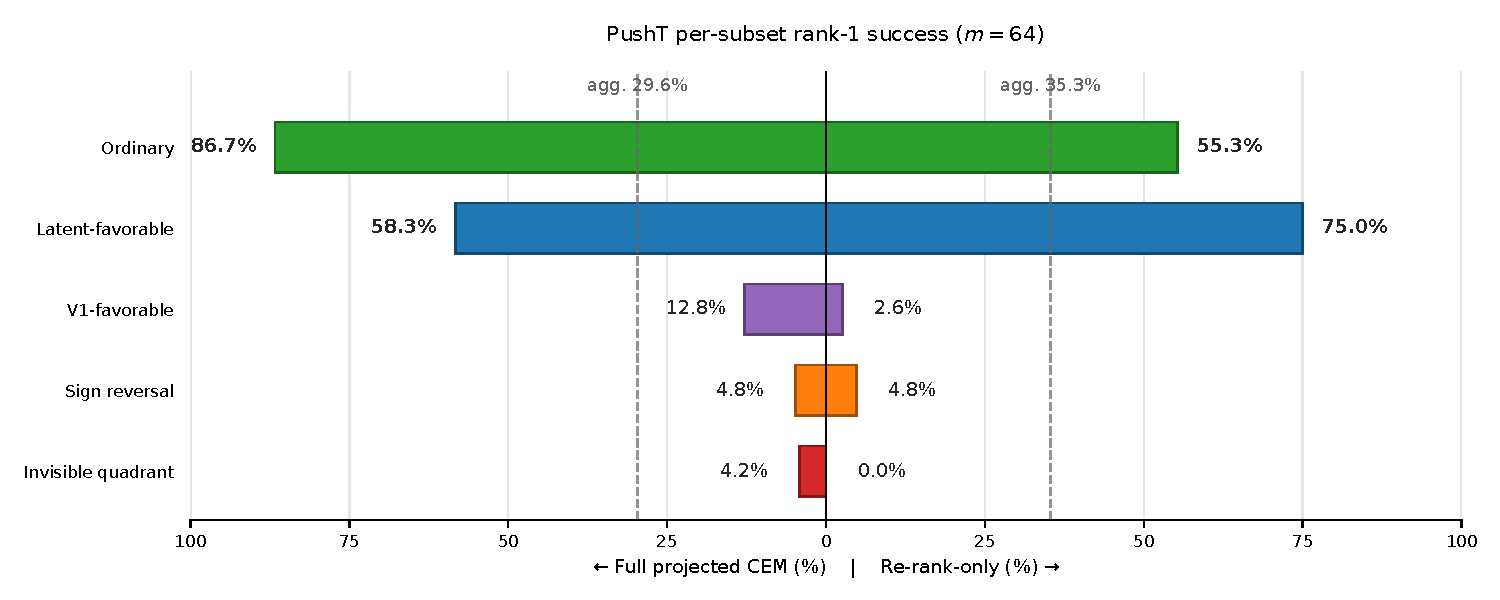
\includegraphics[width=0.9\textwidth]{figures/fig4_butterfly.pdf}
\caption{Per-subset rank-1 planning success at $m = 64$ under two PushT protocols, displayed as a butterfly chart. Left bars show full projected CEM; right bars show re-rank-only. Dashed lines indicate aggregate success. Invisible-quadrant and sign-reversal pairs fail under both protocols, while ordinary and latent-favorable pairs show protocol-dependent differences.}
\label{fig:butterfly_appendix}
\end{figure}

Invisible-quadrant and sign-reversal pairs fail under both protocols.
Ordinary pairs reach 86.7\% under full projected CEM but only 55.3\% under
re-rank-only, suggesting that projected search, not only projected
selection, benefits these pairs.  Latent-favorable pairs show the opposite
pattern: 75.0\% under re-rank-only versus 58.3\% under full projected CEM,
consistent with default CEM producing a better pool for those cases.  This
per-subset decomposition complements the aggregate flatness in
Appendix~\ref{app:stage1b_pusht_rerank} and shows that subset effects
partially cancel in aggregate.

\subsection{Taxonomy Distribution}
\label{app:stage1b_taxonomy}

Across 122 taxonomy cells, the case distribution is A=18, B=8, C=10, E=4,
and unclassified=82.  Case~A, where endpoint geometry transfers to
planning, appears mainly in PushT ordinary and latent-favorable cells at
medium-to-high dimensions.  Case~B, rank-insensitive success, covers Cube
full projected CEM cells; Case~C, endpoint failure as a planning signal,
covers PushT failure subsets.  Case~E, rank-insensitive success in a
locally sufficient pool, is stable: the PushT re-rank-only ordinary subset
passes the tolerant Case~E criterion at $m=64$.  Case~D, emergent local
geometry despite weak endpoint ranking, is not observed.  These categories
instantiate the taxonomy summarized in Table~3.
